\section{Implementação em C}
Nesta seção, buscar-se-á analisar os algoritmos comentados em C a fim de analisar os impactos causados no desempenho quando executado um algoritmo em uma linguagem interpretada, tal como o Python.

Após visto o comportamento dos algoritmos quando implementados em Python, uma linguagem interpretada, percebe-se que, mesmo para vetores pequenos, o tempo gasto para ordená-los é significativo.

Quando implementados utilizando a linguagem C, contudo, percebe-se uma considerável redução na duração dos testes, uma vez que, em razão do C ser uma linguagem compilada, as malhas de repetições tendem a ser mais eficientes.
% TODO por que são mais eficientes?
Ademais, ao utilizar a linguagem C, há um maior controle na forma como o código será executado, devido ao C ser uma linguagem com um nível mais baixo.
% TODO ou seja, ...
Dessa forma, serão analisados os desempenhos de alguns dos algoritmos já implementados em Python, mas, desta vez, estes serão escritos na linguagem C.

A fim de realizar o testes, os algoritmos foram implementados na linguagem C, utilizando, como referência, os códigos já escritos em Python. Sendo assim, tendo em vista que os códigos utilizandos em C não foram otimizados e nem modificados de forma a deixá-los mais lentos, ter-se-á uma comparação equânime.

Além disso, as funções foram invocadas no Python visando criar os gráficos dos resultados.

Foram realizados somentes testes visando analisar o comportamento dos algoritmos em C quando estes são submetidos a listas com tamanhos variáveis, ou seja, o segundo teste não será executado pois..
\newpage
\subsection{Resultados}
\begin{figure}[h]
    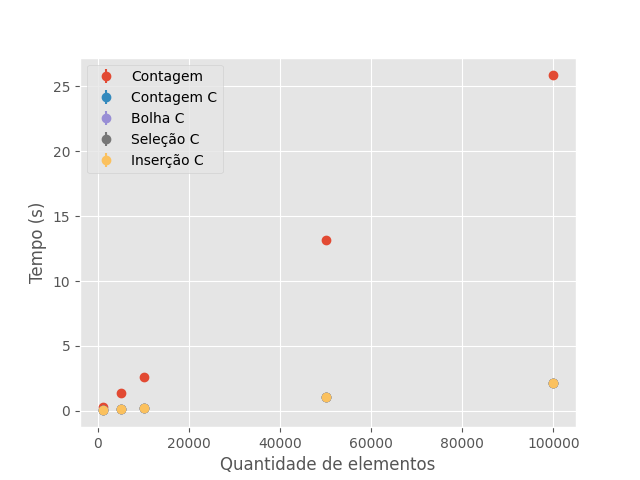
\includegraphics[width=8cm]{c sizes.png}
    \caption{Gráfico ilustrando o tempo médio de execução dos algoritmos implementados em C comparado ao do contagem, implementado em Python.}
\end{figure}
Perceptivelmente, o ganho de desempenho dos algoritmos implementados em C mostrou-se singificativo, mesmo os mais lentos quando implementados em Python, como o bolha, obtiveram uma performance superior ao contagem da linguagem inicial.

De fato, o contagem implementado em C mostrou-se *\% mais eficiente do que a sua versão em Python. Dessa maneira, ....

Ademais, nota-se que, ainda que com listas pequenas, o desempenho dos algoritmos em C em relação aos do Python permaneceu quase constante, isto é, ao aumentar o tamanho das listas, a implementação em C não obteve um ganho nem uma perda expressiva. Consequentemente, ...

Portanto, visando um ganho de performance, é recomendável a utilização da linguagem C a fim de implementar algoritmos que se "aproveitam" de malhas de repetições.
Caso seja necessário o uso do Python para outras tarefas no projeto, as funções em C podem ser chamadas por meio de ...
